\chapter{Supplemental Information}
\label{supplementals}

% Software list/table
% DeepLabCut \href{https://github.com/DeepLabCut/DeepLabCut}
% MWorks \href{https://mworks.github.io}
% ScanImage 2016 \href{http://scanimage.vidriotechnologies.com}

\section{Supplementary Tables}

\begin{table}[ht]
  \caption{Software and Available Repositories}
  \centering
  \footnotesize
  \begin{tabular}{ p{1.8cm}p{7.7cm}p{3.9cm}  }
    \toprule
    Resource & Source & Publications \\
    \midrule
    OpenRatBox  & https://github.com/coxlab/behavior\_rig & N/A \\ 
                & https://github.com/coxlab/protocols & N/A \\ 
                & https://github.com/julianarhee/trainingtracker & N/A \\ 
    \midrule
    Custom Stimuli & https://github.com/julianarhee/morph-pov & N/A \\
                   & https://github.com/coxlab/povray & \citet{Zoccolan2009} \\
    POVRay  & http://www.povray.org & N/A \\
    MWorks  & https://mworks.github.io & N/A \\
    \midrule
    Retinotopic Mapping & https://github.com/julianarhee/retinotopy-mapper & N/A \\ 
                        & https://github.com/zhuangjun1981/retinotopic\_mapping & \citealt{Zhuang2017}\\
    \midrule
    ScanImage   & http://scanimage.vidriotechnologies.com & \citet{Pologruto2003} \\ 
    \midrule
    2p Processing  & https://github.com/julianarhee/acquisition-tools & N/A \\ 
                   & https://github.com/HarveyLab/Acquisition2P\_class & N/A \\
                   & https://github.com/HarveyLab/helperFunctions & N/A \\
    CaImAn & https://github.com/flatironinstitute/CaImAn  & \citet{Giovannucci2019,Pnevmatikakis2019} \\
    Suite2p & https://github.com/mouseland/suite2p & \cite{Pachitariu2017} \\
    \midrule
    DeepLabCut   & https://github.com/DeepLabCut/DeepLabCut & \citet{Mathis2018,Nath2019} \\
    \midrule
    Scikit Learn   & https://scikit-learn.org & \citet{Pedregosa2011} \\
    \bottomrule
  \end{tabular}
  \label{tab:software}
\end{table}


%http://n2t.net/addgene:104488; RRID:Addgene_104488

% Data numbers 
\begin{table}[h]
  \caption{Data Summary}
  \centering
  \begin{tabular}{lllll}
    \toprule
    Stimulus & Area & Rats & FOVs & Responsive or Fit Cells   \\
    \midrule
    Moving bar & V1  & 7 & 9 & 1277        \\
               & LM  & 7 & 9 & 530         \\
               & LI  & 6 & 9 & 502          \\
    \midrule
    Receptive Fields & V1  & 11 & 11 & 548  \\
                     & LM  & 8 & 8 & 241   \\
                     & LI  & 10 & 10 & 279    \\
    \midrule
    Gratings & V1  & 7 & 7 & 2211     \\
             & LM  & 8 & 8 & 2084     \\
             & LI  & 7 & 7 & 966     \\
    \midrule
    Objects  & V1  & 9 & 8 & 1028   \\
             & LM  & 10 & 7 & 684   \\
             & LI  & 8 & 7 & 402    \\
    \bottomrule
  \end{tabular}
  \label{tab:data_counts}
\end{table}

\clearpage

\section{Supplementary Figures}

% \section{Related to Chapter 1}
\begin{figure}[hbt!]
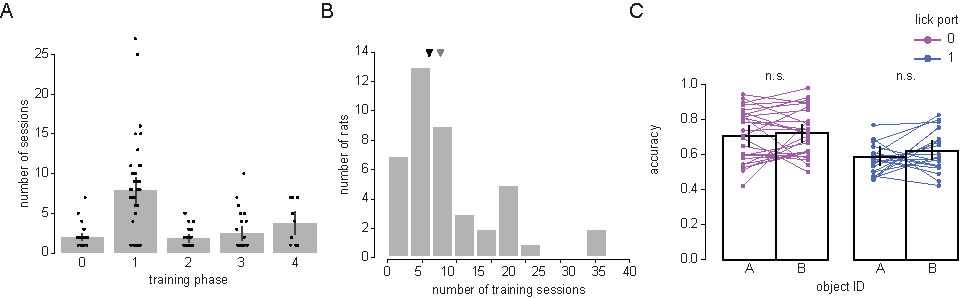
\includegraphics[width=\textwidth]{figures/supplemental/fig_s1_aggregate_training/fig_s1_aggregate_training.pdf}
    \vspace{.1in}
    \caption[Aggregate training data]{Aggregate training data. 
    \textbf{A.} Number of sessions per training phase. Each dot represents one rat. Bars show mean and SD.
    \textbf{B.} Histogram of the total number of training sessions to reach criterion (across all phases). Black and gray triangles denote the mean and median, respectively. 
    \textbf{C.} Accuracy split by object identity (object 1 or object 2) and port mapping (whether to lick right for object 1 and lick left for object 2, or vice versa). Each pair of lines represents one rat. Colors indicate arbitrary port assignment for the standard 2-object class paradigm. 
    \label{supfig:aggregate_training}}
\end{figure}


% FIGURE S.2 MORPH
\begin{figure}
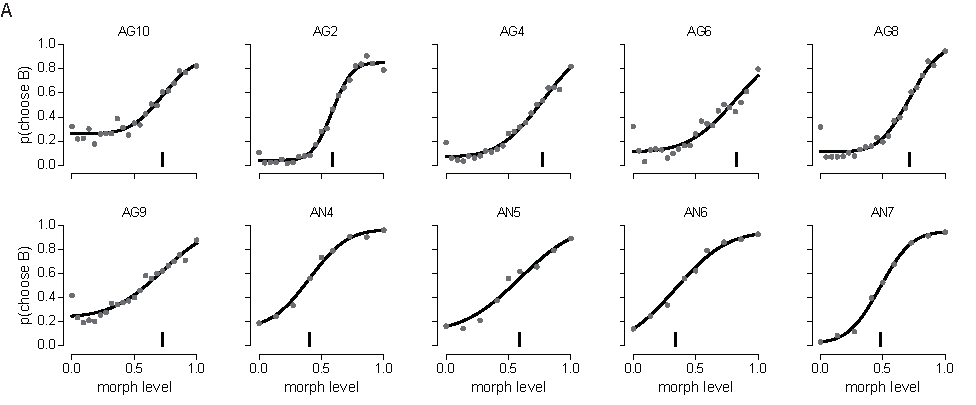
\includegraphics[width=\textwidth]{figures/supplemental/fig_s2_morphs_per_animal/fig_s2_morphs_per_animal.pdf}
    \caption[Individual psychometric curves]{Individual psychometric curves for morphs. 
    \textbf{A.} Example psychometric curves for n=10 out 13 rats that passed criterion performance (70\% accuracy on the basic discrimination of the anchors). Each dot represents the fraction of times the animal chose the ``B''-assigned port, where morph level 0 is 0\%B and morph level 100 is 100\%B. Solid curves are the fits, vertical lines indicate bias. 
    \label{supfig:morphs}}
\end{figure}

% FIGURE S.3 INVAR
\begin{figure}[t!]
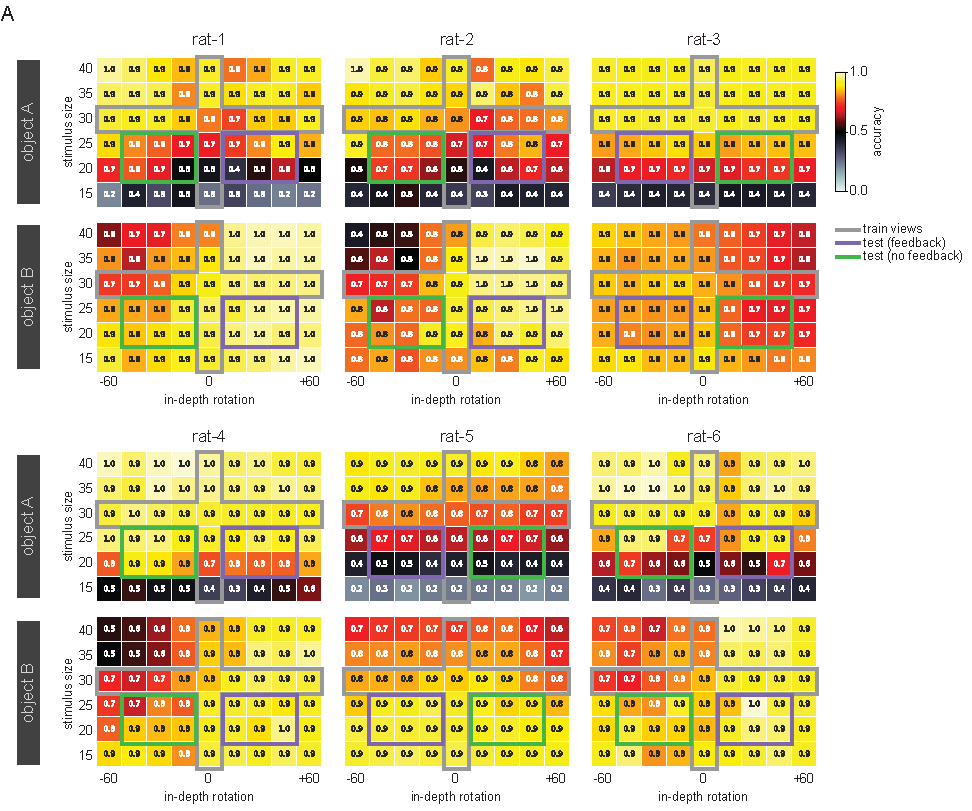
\includegraphics[width=\textwidth]{figures/supplemental/fig_s3_heatmaps_per_rat/fig_s3_heatmaps_per_rat.pdf}
    \caption[Individual invariance performance]{Individual performance on invariance test.
    \textbf{A.} Performance data for an example group of n=6 rats, split by object ID (top=object A, bottom=object B) and stimulus transformation. Colormap indicates accuracy. Gray, initial training views (views in which only a single transformation axis changes, size or rotation). Purple, views for which no feedback was provided. Green, size-matched view for which feedback was provided. 
    \label{supfig:heatmaps}}
\end{figure}

% \section{Related to Chapter 3}
% FIGURE S.4 STIMULI
\begin{figure}[t!]
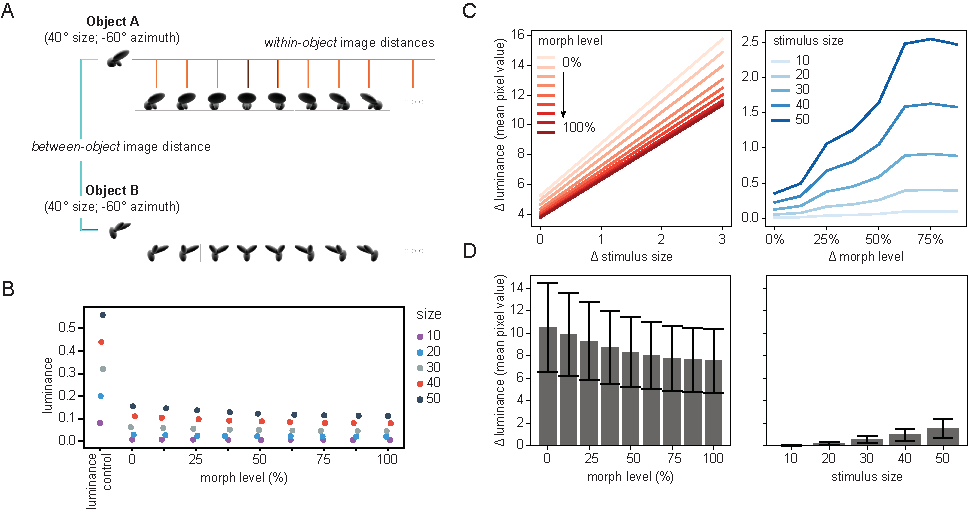
\includegraphics[width=\textwidth]{figures/supplemental/fig_s4_stimulus_metrics/fig_s4_stimulus_metrics.pdf}
    \vspace{.1in}
    \caption[Stimulus metrics]{Metrics defining the differences between images.
    \textbf{A.} The two objects were specified to have larger within-object distances than between-object distances at a given view (adapted from \cite{Zoccolan2009}). Distance was calculated as the Euclidean distance between the images. 
    \textbf{B.} Global mean luminance for each object image used for two-photon experiments, calculated as the average pixel value across the screen (image was transformed to screen coordinates), normalized by the max luminance value (255). Images are subsets of the images used to test behavior in trained rats. Luminance controls were full field stimuli (no shapes) assigned constant grayscale values that were experimentally determined to match photometer measurements of the screen at each stimulus size (placed at the position of the animal's eye). 
    \textbf{C.} \textit{Left}: Within-morph differences across different sizes. For each morph image, this was calculated as the pixel-wise difference between the morph at size \textit{s1} and the same morph at size \textit{s2}, for each pair of neighboring sizes. Level 1 represents the two smallest sizes, while level 4 represents the two largest sizes. Shades of red correspond to morph levels ordered from 0\%B to 100\%B. |textit{Right}:  Between-morph differences at each size. For each size (shades of blue), this was calculated as the pixel-wise difference between morph \textit{m0} at size \textit{s} and morph \textit{m1} at the same size, for each neighboring morph. Differences are greater at larger sizes.
    \textbf{D.}. Average within-morph differences (across size) for each morph tested (left), and average between-morph differences (across morph levels) for each size tested (right).    
    \label{supfig:stimulus_metrics}}
\end{figure}

% Visual field targeting
\begin{figure}[t!]
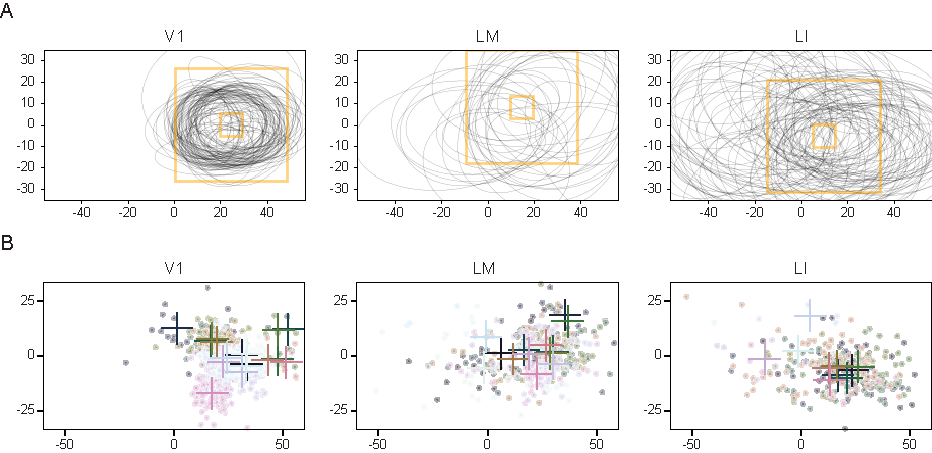
\includegraphics[width=\textwidth]{figures/supplemental/fig_s5_vf_targeting/fig_s5_vf_targeting.pdf}
    \vspace{.1in}
    \caption[Visual Field Targeting]{Targeted visual stimulation with receptive field mapping.
    \textbf{A.} Receptive fields of all cells in an example V1 FOV (left), LM (middle), and LI (right) FOV. Yellow boxes correspond to the bounding boxes around the smallest and largest stimulus sizes targeted to the center-of-mass of the receptive fields.
    \textbf{B.} Receptive field centers plotted in screen coordinates and corresponding center-of-mass estimates for each FOV included in the object analyses (Chapter 4) for V1 (left), LM (middle), and LI (right). Colors are different imaging sites. Dots correspond to receptive field centers of cells and crosses are the corresponding center-of-mass estimates for the dots of the same color.
    \label{supfig:vf_targeting}}
\end{figure}


% \subsection{Comparison of stimulus size for receptive field measurements}
\begin{figure}[tp!]
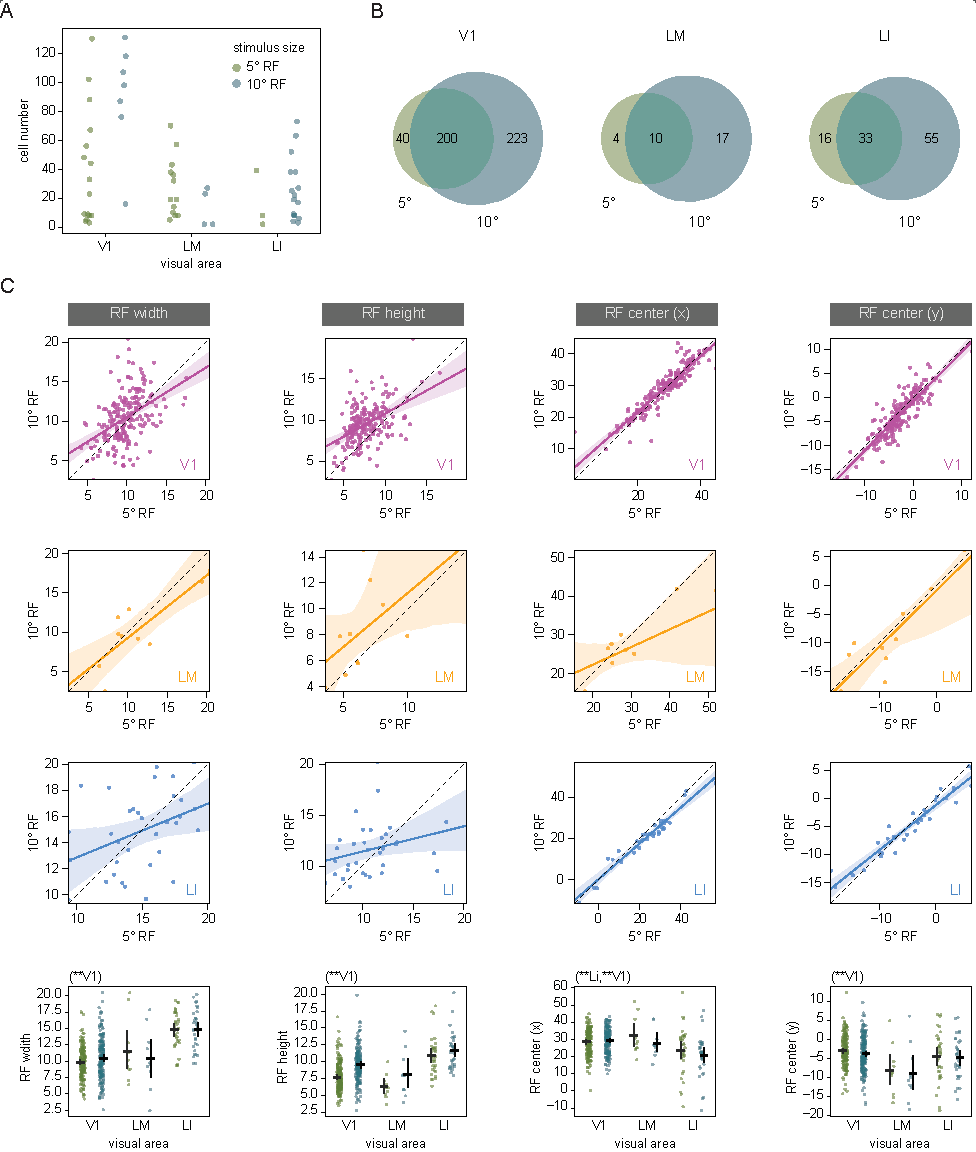
\includegraphics[width=\textwidth]{figures/supplemental/fig_s6_rf5_v_rf10/fig_s6_rf5_rf10.pdf}
    \caption[RF mapping stimuli]{RFs measured with 2 stimulus sizes.
    \textbf{A.} Number of cells with well-fit RFs (see Methods) for \ang{5} (light green) and \ang{10} (dark green) tile sizes. Each dot is an imaging site.
    \textbf{B.} RF counts for FOVs in which both tile sizes were tested for V1 (left), LM (middle), and LI (right). Overlap, cells fit with both sizes. Light green, \ang{5}. Dark green, \ang{10}.
    \textbf{C.} Scatter plots of RF parameters from fits using the \ang{5} (x-axis) and \ang{10} (y-axis) for cells fit with both. Columns represent estimated parameters of the 2-D Gaussian ($\sigma_x$, $\sigma_y$, $x_0$, $y_0$). Row 1 (magenta): V, Row 2 (orange): LM, Row 3 (blue): Li. Row 4, scatterplot data plotted side-by-side for the parameter in the column (\ang{5}: light green, left, \ang{10}: dark green, right) for each area. Axis titles above Row 4 plots indicate visual areas for which there was a significant difference between stimulus sizes (Wilcoxon rank test, *:p<0.05, **:p<<0.01).
    \label{supfig:rf5_rf10}}
\end{figure}

% \subsection{Comparison of stimulus size for receptive field measurements}
\begin{figure}[tp!]
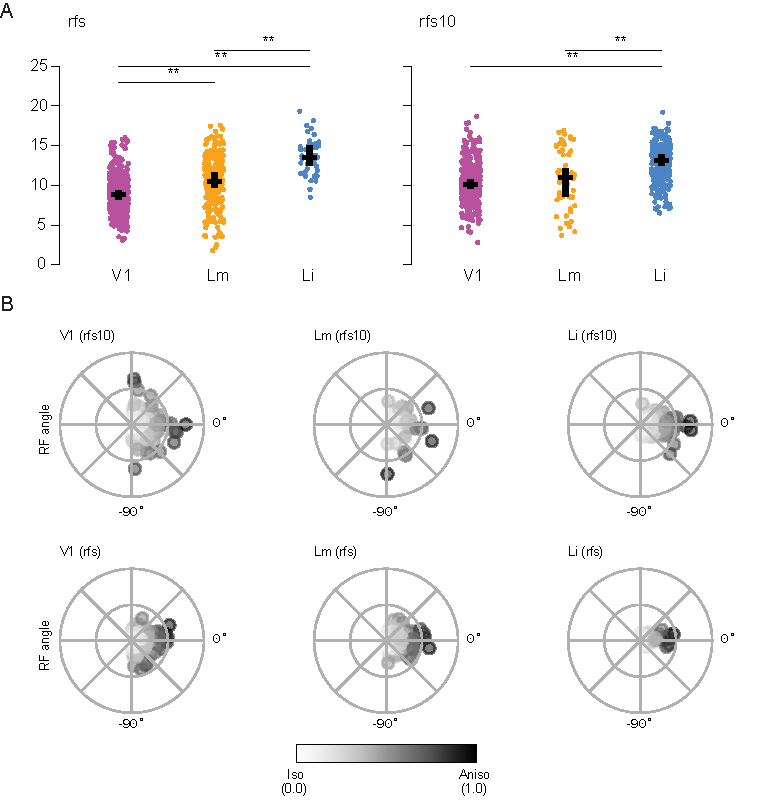
\includegraphics[width=\textwidth]{figures/supplemental/fig_s7_rf5_rf10_aggregate/fig_s7_rf5_rf10_aggregate.pdf}
    \caption[RF mapping stimuli]{RFs measured with 2 stimulus sizes.
    \textbf{A.} Number of cells with well-fit RFs (see Methods) for \ang{5} (light green) and \ang{10} (dark green) tile sizes. Each dot is an imaging site.
    \textbf{B.} RF counts for FOVs in which both tile sizes were tested for V1 (left), LM (middle), and LI (right). Overlap, cells fit with both sizes. Light green, \ang{5}. Dark green, \ang{10}.
    \textbf{C.} Scatter plots of RF parameters from fits using the \ang{5} (x-axis) and \ang{10} (y-axis) for cells fit with both. Columns represent estimated parameters of the 2-D Gaussian ($\sigma_x$, $\sigma_y$, $x_0$, $y_0$). Row 1 (magenta): V, Row 2 (orange): LM, Row 3 (blue): Li. Row 4, scatterplot data plotted side-by-side for the parameter in the column (\ang{5}: light green, left, \ang{10}: dark green, right) for each area. Axis titles above Row 4 plots indicate visual areas for which there was a significant difference between stimulus sizes (Wilcoxon rank test, *:p<0.05, **:p<<0.01).
    \label{supfig:rf5_rf10_aggregate}}
\end{figure}


% \subsection{Demonstration of spherical correction}
\begin{figure}[t!]
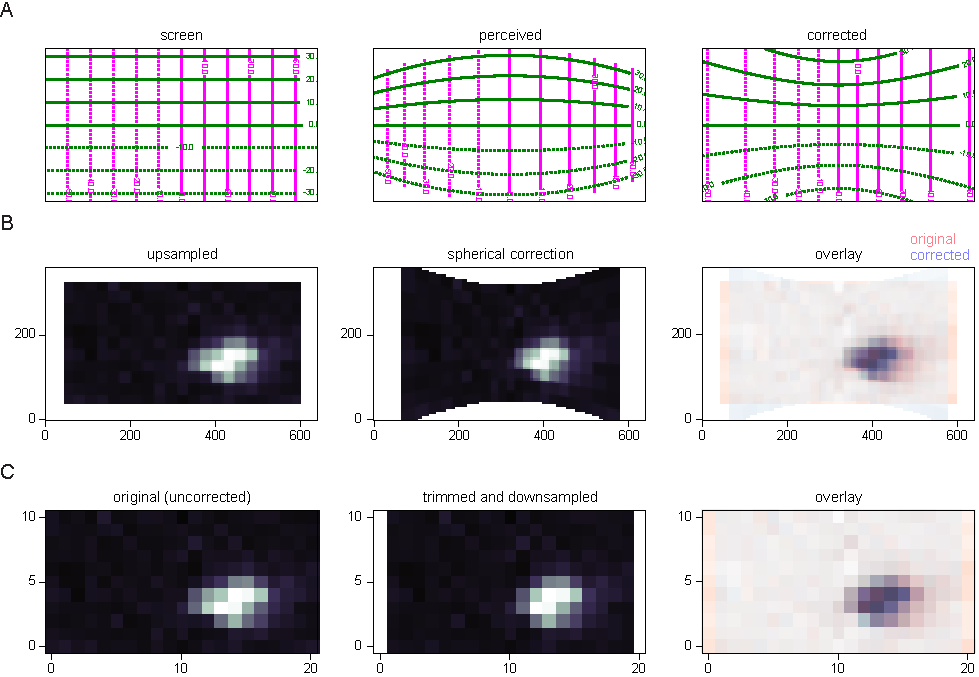
\includegraphics[width=\textwidth]{figures/supplemental/fig_s8_spherical_correction_steps/fig_s8_spherical_correction_steps.pdf}
    \vspace{.1in}
    \caption[Spherical correction]{Steps for posthoc spherical correction.
    \textbf{A.} Screen coordinates of the monitor in degrees of visual angle. Green, isoelevation lines. Magenta, isoazimuth. \textit{Middle}: Estimate of what the animal perceives without spherical correction. \textit{Left}: Transform to warp RF responses measured without spherically-corrected stimuli. 
    \textit{B.} Steps for spherically correcting measured RF responses. First, the measured RF array, corresponding to the cell's average response to each stimulated position, is transformed to pixel coordinates (left, downsampled screen resolution is upsampled RF array). Then, the transformation shown in \textbf{A} is applied to the RF array (middle). The overlay (right) shows the warped RF array (blue) overlaid on the original RF array (red) in pixel coordinates.
    \textit{C.} Steps to convert spherically-corrected RF ararys back to coordinates of the tiled RF map. Left, the original RF array showing the cell's response to each of the tiled position. Middle, The upsampled and warped RF array (middle panel directly above in \textbf{B}) is then trimmed and downsampled back to the tiled position coordinates (as opposed to the upsampled pixel coordinates). Right, overlay of the ``corrected'' RF array (blue) ontop of the origin RF array (red).
    \label{supfig:spherical_correction_steps}}
\end{figure}

% \subsection{Spherical correction, examples}
\begin{figure}[t!]
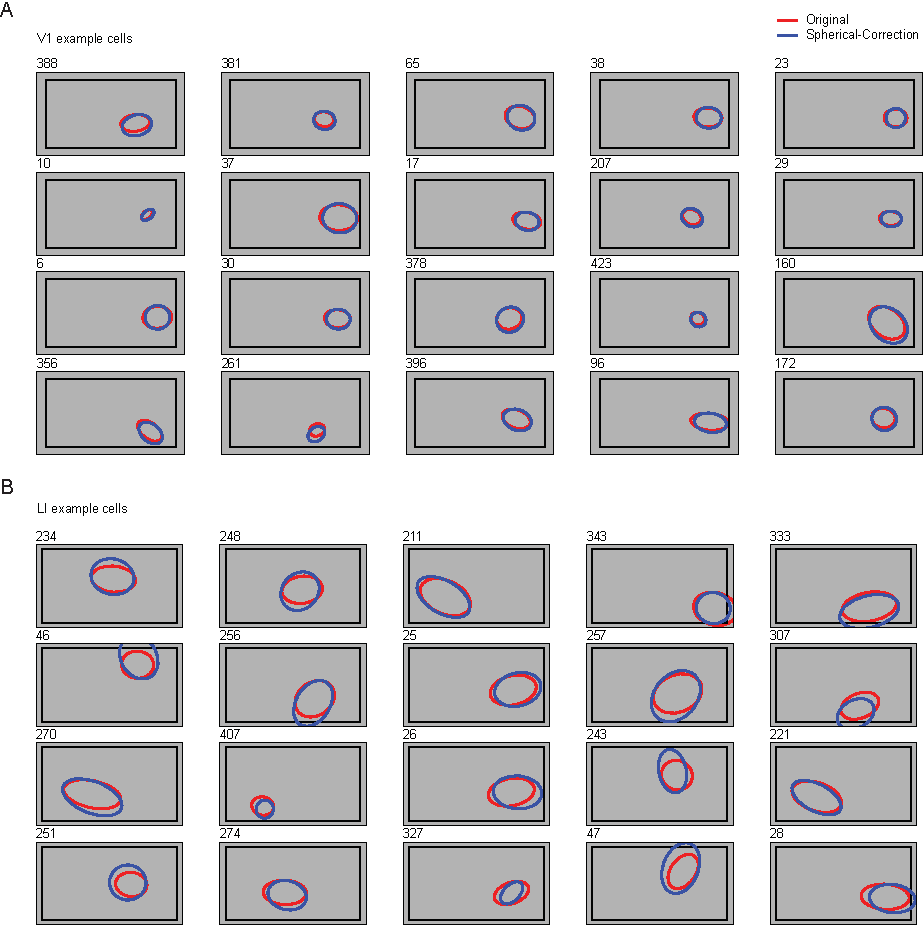
\includegraphics[width=\textwidth]{figures/supplemental/fig_s9_spherical_correction_examples/fig_s9_spherical_correction_examples.pdf}
    \vspace{.1in}
    \caption[Example RFs after spherical correction]{Example receptive field fits before and after spherical correction.
    \textbf{A.} Top 30 cells (ranked by goodness-of-fit measure, coefficient-of-determination $R2$) for an example V1 FOV. Red, original RF fit. Blue, RF fit after warping. 
    \textbf{B.} Same as \textbf{A}, but for an example LI FOV, where cells are generally larger and cover peripheral parts of the screen.
    \label{supfig:spherical_correction_examples}}
\end{figure}


% \subsection{Spherical correction, aggregate}
\begin{figure}[t!]
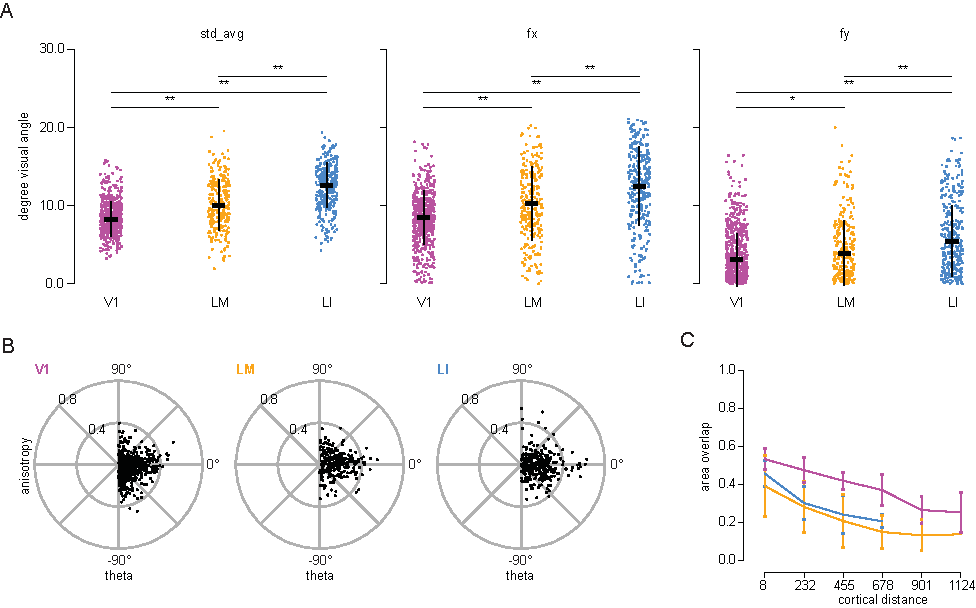
\includegraphics[width=\textwidth]{figures/supplemental/fig_s10_spherical_correction_aggregate/fig_s10_spherical_correction_aggregate.pdf}
    \vspace{.1in}
    \caption[RF properties after spherical correction]{Receptive field properties after spherical correction. 
    \textbf{A.} Average size (left), measured as half-width at half-max (HWHM) of a fit 2D-Guassian. Also shown is the projection of the major axis of each ellipse onto the horizontal (middle) and vertical (right) axes of visual space for each cell. Each dot represents one cell. Horizontal and vertical bars, mean and SD across cells. 
    \textbf{B.} Anisotropy, measured as the ratio of major to minor axes of the fit ellipse, as a function of receptive field angle. Each dot is a cell. Anistropy ranges from 0 to 1, where 0 represents perfectly isotropic receptive fields (a circle), and 1 represents an extremely linear receptive field. Receptive field angles of 0 represent orientations parallel to the horizontal axis, and 90 degrees represents orientation parallel to the vertical axis.
    \textbf{C.} Receptive field overlap as a function of cortical distance. For each pair of cells, overlap is measured as the intersection of their receptive fields divided by their union. Error bars, SD.  
    \label{supfig:spherical_correction_aggregate}}
\end{figure}

% \subsection{Comparison of receptive field and gratings tuning}
\begin{figure}[t!]
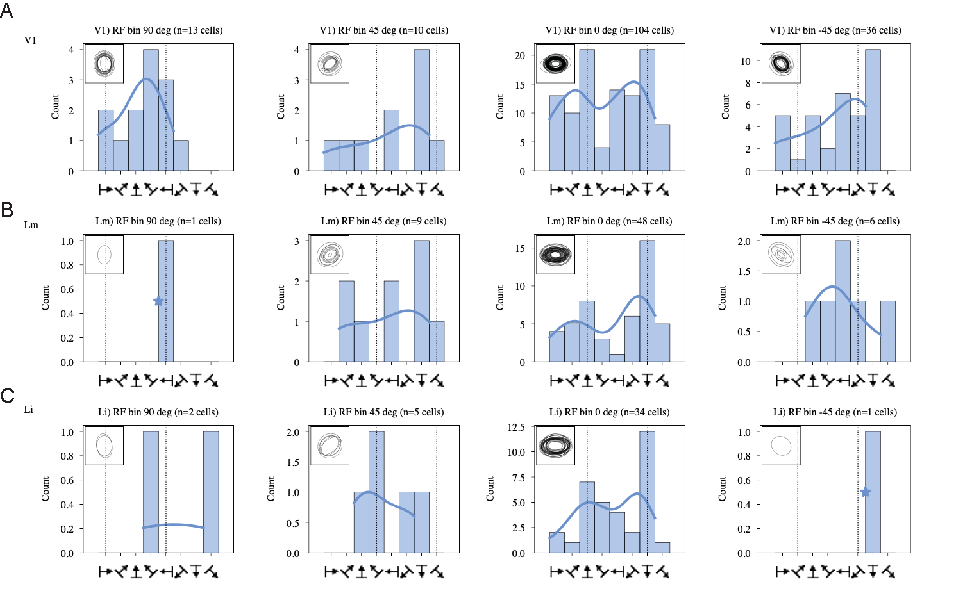
\includegraphics[width=\textwidth]{figures/supplemental/fig_s11_theta_vs_rf/fig_s11_theta_vs_rf.pdf}
    \vspace{.1in}
    \caption[Direction selectivity and RF orientation]{Direction selectivity by receptive field orientation.
    \textbf{A.} Distributions of preferred theta (direction of motion) for cells with well-fit direction tuning curves and well-fit RFs (see Methods), split by binned RF orientation, for V1 cells. Inset at the upper left of each subplot shows the actual RF fits for the cells whose preferred theta distributions are shown in the corresponding histogram. Solid curves, estimated KDEs (kernel density estimates). 
    \textbf{B.} Same as \textbf{A}, but for LM cells. Plots with a single star (and no KDE curve) contain only 1 cell. 
    \textbf{C.} Same as \textbf{A} and \textbf{B} for LI cells. Conventions as above.
    \label{supfig:theta_vs_rf}}
\end{figure}



% \section{Related to Chapter 4}
\begin{figure}[t!]
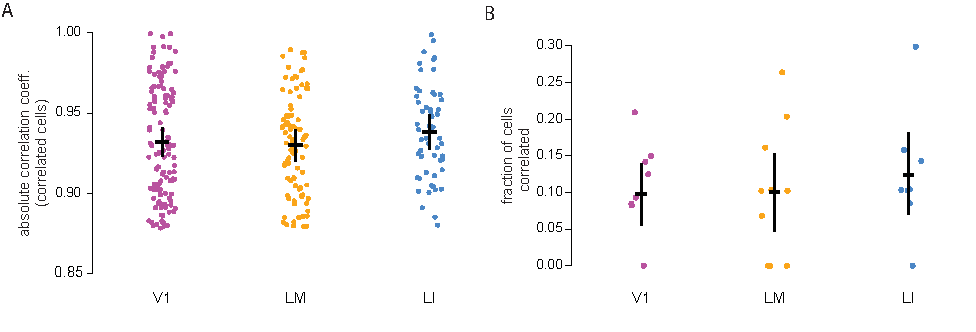
\includegraphics[width=\textwidth]{figures/supplemental/fig_s12_luminance_corr/fig_s12_luminance_corr.pdf}
    \vspace{.1in}
    \caption[Luminance and size tuning]{Relationship between luminance selectivity and size selectivity.
    \textbf{A.} Distributions of absolute values of correlation coefficients for cells with significant relationships between size tuning and luminance tuning (Pearson's, p<0.05) for visually responsive cells in V1, LM, and LI. Each dot represents one cell. Vertical and horizontal bars, mean and SD. 
    \textbf{B.} Fraction of cells with significant correlations for each visual area recorded in V1, LM, and LI. Each dot represents one imaging site.  
    \label{supfig:luminance_corr}}
\end{figure}

% \subsection{Tuning similarity as a function of distance}

% \subsection{Classifier accuracy as a function of receptive overlap}

% \subsection{Classifier generalization, matched for receptive field size}
